
\chapter{Crawl.js} % Main chapter title
In this chapter we describe how crawl.js splits and distributes the work in detail.
\label{Chapter4} 
\lhead{Chapter 4. \emph{Crawl.js}} 

\section{System overview}
Crawl.js is a decentralized system. Each \emph{worker} in the system is standalone and autonomous and does not depend on any other worker. The only thing a worker needs is a connection to the \emph{Queues} and the \emph{Stores}. Figure~\ref{system_overview} gives an overview of the main components in the system.

Lets follow the path of an URL in the system.
The first thing a worker needs to do is get some URLs (1) from a remote queue (Note that the worker knows by his own which Queue to ask). Step 2 and 3 involves fetching, parsing and storing the content given by the URL. Thanks to the asynchronous nature (Streaming) of Crawl.js the parsing (3) can happen before the fetching (2) is done. Even storing the content (3) is done while fetching. More on this later. Whenever a new URL is extracted in the parsing step it is added to the \emph{Queue}. The queue then decides what to do (\emph{4a},\emph{4b}). Either it is kept in the local (in-memory) queue or dipatched to a remote one (batch processing).

\begin{figure}[h]
\centering
  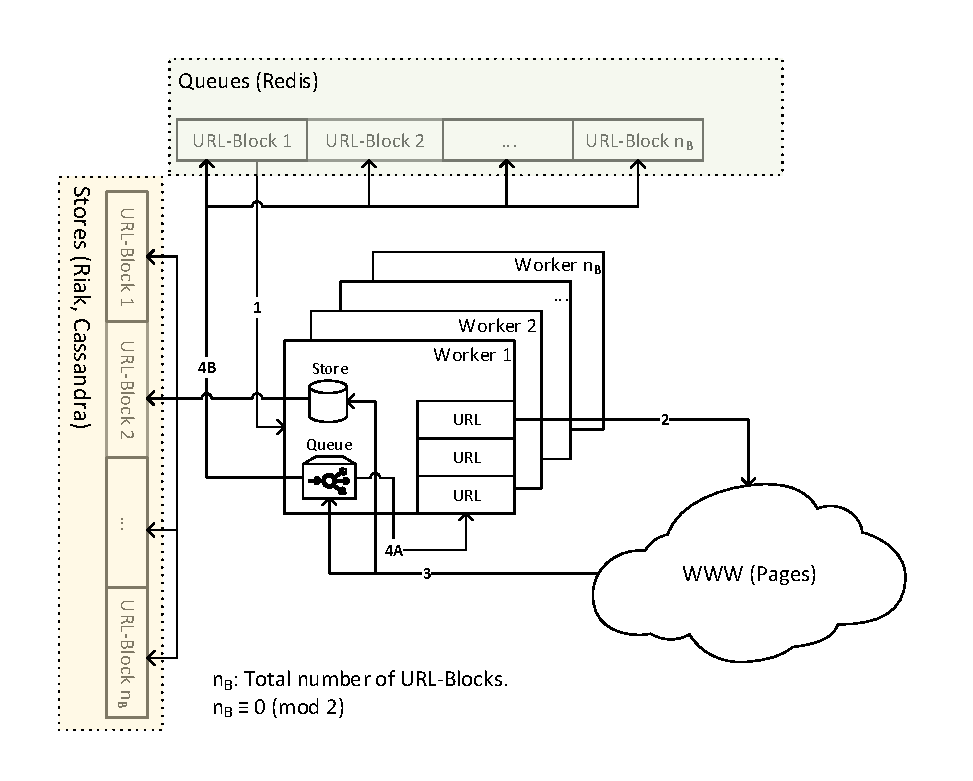
\includegraphics[width=1\textwidth]{Figures/system_overview.pdf}
\caption{Crawl.js - System Overview}
\label{system_overview}
\end{figure}

\section{Queues}
Queues play a central role in the Crawl.js system. There are \emph{local} queues (in-memory) and \emph{remote} queues. At any time each worker is able to identify the responsible queue for a given URL without any communication to other components in the system. This feature is what makes the system decentralized and is discussed in a seperate section (\emph{Dispatcher}) in detail.

\subsection{Queue}
First a few words about how we use the word \emph{Queue} within this document. Strictly and technically speaking it is \emph{more} than a queue. A basic queue has the following operations:
\begin{itemize}
  \item enqueue
  \item dequeue
\end{itemize}

New items are enqueued at the bottom of the list and existing items are dequeued from the top. In terms of URLs this could work. But, what if we want to prioritize the URLs in the queue in some way. Of course we could enqueue URLs in the order we want them prioritiezed but this is rather inconvinient and does not work for existing URLs in the queue. We want to be able to re-prioritize (remove/change) existing URLs in the queue. And as mentioned in \cite{hp_crawler} fetching URLs in the order they were enqueued is a bad idea because of second-level locality in the links.

Therefore in Crawl.js a queue is a \emph{sorted set}. With sorted sets we can achieve whatever order we like. We can simulate a queue with it (thats why we still call it queue), use a pure random approach (set) or use custom algorithms to compute the order in the queues (re-visit policies).

\subsection{Local Queue (in-memory)}
As the title describes it, from the worker's point of view it is a local and in-memory queue.

\subsection{Remote Queue (Redis.io)}

\subsection{Dispatcher}

\subsection{URL-Block}
A URL-Block is nothing more than a set of URLs or to be more precise a queue of URLs. It is obvious that at some point we will need some ordering within the set of URLs.
This queue or URL-Block is the entity used to distribute the work. There is always only one consumer (worker) per URL-Block.
This fact of a 1:1 association between a URL-Block and a worker (consumer) is a design choice and we will discuss the dis-/advantages later.

\section{Stores}
Ola store
\subsection{Implementation (Riak)}

\section{Worker (a crawl.js instance)}
A worker is autonomous and responsible for one URL-Block. Why autonomous? Because a worker can fetch pages, store them and extract new URLs out of it. Newly found URLs are assigned (\emph{Mapper}) to their URL-Block and dispatched automatically. All this happens without any interaction to other components in the system. This keeps the number of inter-communication messages very low.

One worker for one URL-Block. This is true for consuming URLs but obviously we have multiple URL producers. Namely each worker in the system is a candidate for producing new URLs because each one is able to assign and dispatch newly found URLs independly. So we have one consumer and multiple producers whithin one URL-Block (queue).
\subsection{States}
Dummy
\subsection{Software Architecture}
Dummy
\subsection{Configuration}
Dummy
\subsection{github}
Dummy
\subsection{Performance}
Dummy
\subsection{Storage}
Dummy
\subsection{Details - (Url-normalization, ..)}

